Le comportement créé permet de remplir tous les objectifs énoncés par le cahier des charges, à savoir l'exploration d'un environnement inconnu dans le but d'y repérer des <<sources>> marquées par des taches noires au sol et l'exploitation de ces sources, tout en évitant les obstacles éventuels et en gérant adéquatement l'autonomie des robots. De plus, l'arène a aussi dû être créée afin de convenir à l'expérience ainsi qu'aux spécifications données. Enfin, comme demandé, une évaluation des performances du comportement a été faite. Cette évaluation est présentée ci-dessous.

\section{Evaluation des performances}

\subsection{Efficacité de l'exploitation}

Nous avons d'abord évalué les performances de l'exploitation seule, en donnant au robots la connaissance des sources présentes. Les indicateurs utilisés sont le nombre moyens de trajets totaux et par source, après 10.000 steps, en fonction du nombre de robots, et le nombre de trajets totaux par robot après 10.000 steps. Ceci permet de juger de l'efficacité du déplacement mais aussi du choix de ressource à exploiter. A cet effet, nous utilisons volontairement une répartition de source assez déséquilibrée.
\begin{figure}[htbp]
  \centering
  \includegraphics[width=0.7\textwidth]{pics/initArenaNames.png}
  \caption{Configuration utilisée et référence des sources}
\end{figure}

\begin{figure}[htbp]
\centering
\begin{subfigure}[h!]{0.45\textwidth}
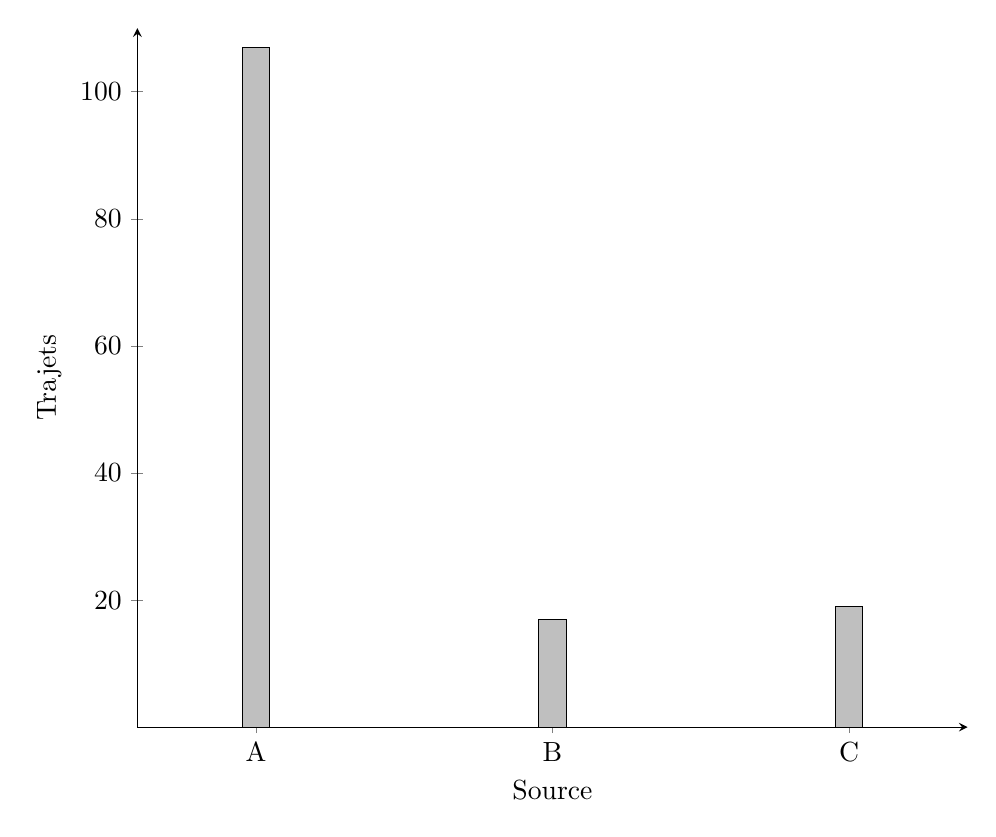
\begin{tikzpicture}
        \begin{axis}[width=\textwidth,
            symbolic x coords={A,B,C},
            xtick=data,
            ymin=0,
            ymax=110,
            xlabel=Source,
            ylabel=Trajets,
            ytick={20,40,60,80,100},
                  axis x line=bottom,
      axis y line=left,
      enlarge x limits=0.2,
          ]
            \addplot[ybar,fill=black!25] coordinates {
                (A,   107)
                (B,  17)
                (C,   19)
            };
        \end{axis}
\end{tikzpicture}
\caption{5 footbots}
\end{subfigure}\hfill\begin{subfigure}[h!]{0.45\textwidth}
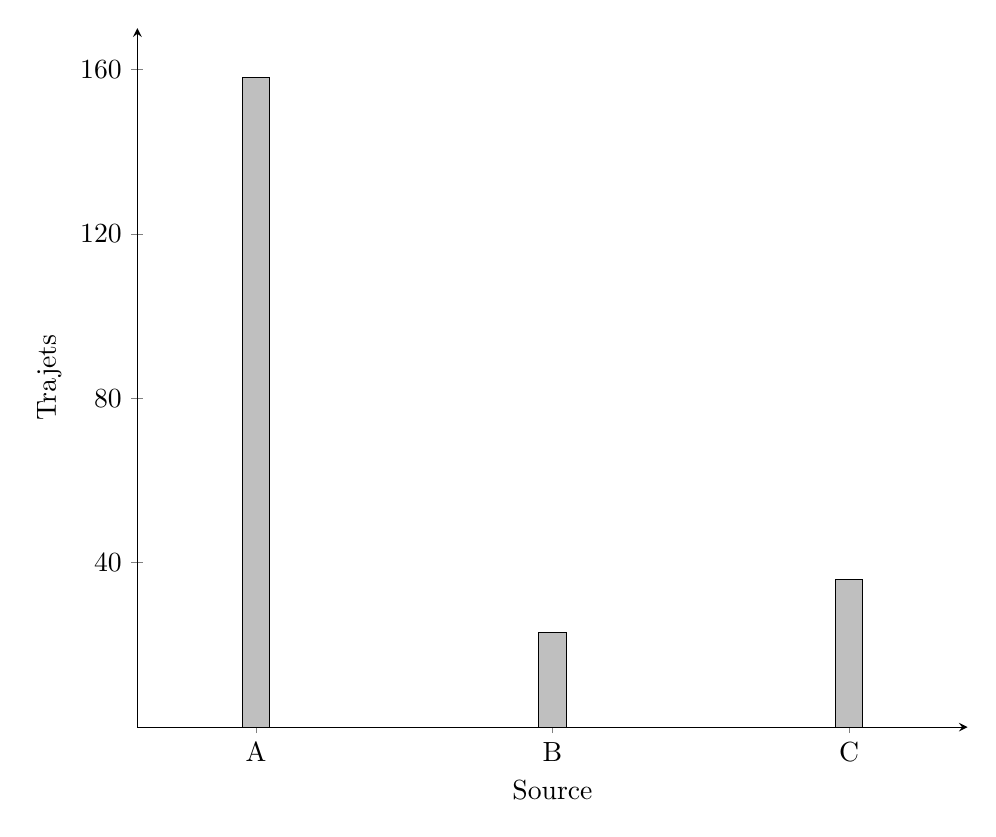
\begin{tikzpicture}
\begin{axis}[width=\textwidth,
symbolic x coords={A,B,C},
xtick=data,
ymin=0,
ymax=170,
xlabel=Source,
ylabel=Trajets,
ytick={40,80,120,160},
      axis x line=bottom,
      axis y line=left,
            enlarge x limits=0.2,
]
\addplot[ybar,fill=black!25] coordinates {
(A,   158)
(B,  23)
(C,   36)
};
\end{axis}
\end{tikzpicture}
\caption{10 footbots}
\end{subfigure}

\vspace{1em}

\begin{subfigure}[htbp]{0.45\textwidth}
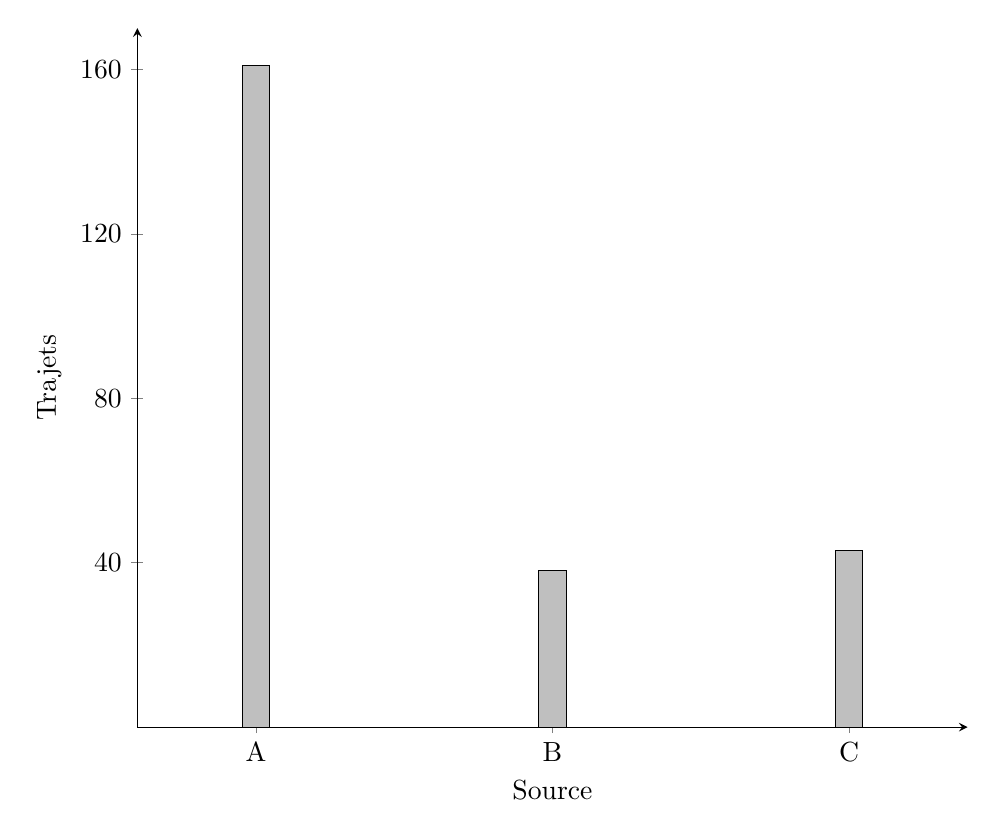
\begin{tikzpicture}
\begin{axis}[width=\textwidth,
symbolic x coords={A,B,C},
xtick=data,
xlabel=Source,
ylabel=Trajets,
ymin=0,
ymax=170,
ytick={40,80,120,160},
      axis x line=bottom,
      axis y line=left,
            enlarge x limits=0.2,
]
\addplot[ybar,fill=black!25] coordinates {
(A,   161)
(B,  38)
(C,   43)
};
\end{axis}
\end{tikzpicture}
\subcaption{15 footbots}
\end{subfigure}
\caption{Nombre de trajets effectués par source au bout de 10000 steps, selon le nombre de robots}
\end{figure}

\begin{figure}[htbp]
\centering
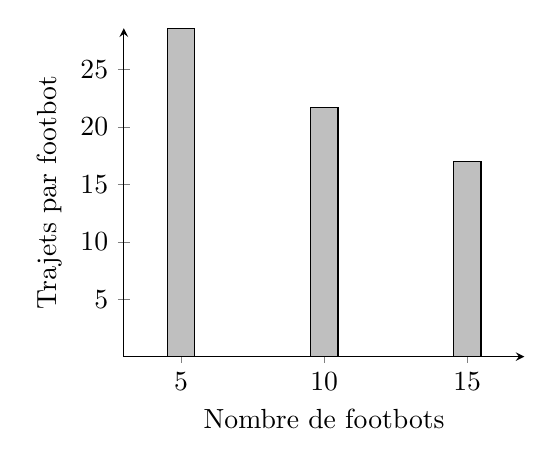
\begin{tikzpicture}
\begin{axis}[width=0.55\textwidth,
symbolic x coords={5,10,15},
xtick=data,
xlabel=Nombre de footbots,
ylabel=Trajets par footbot,
ymin=0,
ytick={5,10,15,20,25},
      axis x line=bottom,
      axis y line=left,
            enlarge x limits=0.2,
]
\addplot[ybar,fill=black!25] coordinates {
(5,   28.6)
(10,  21.7)
(15,   17)
};
\end{axis}
\end{tikzpicture}
\caption{Nombre de trajets effectués par footbot au bout de 10000 steps, selon le nombre de footbots}
\end{figure}

On voit que les robots sont effectivement capables de distinguer la source la plus rentable, mais que l'indice de qualité d'une source utilisé par la décision $\varepsilon$-greedy est peut-être inadapté. En effet, lorsqu'on augmente le nombre de robots, on n'assiste à une meilleure répartition des robots sur les trois sources mais ce n'est pas suffisant. En effet, les robots continuent à utiliser massivement la source A la plus proche, au point que celle-ci n'est visiblement plus rentable car les robots embouteillent complètement la zone entre le nid et cette source. La conséquence directe est que le rendement par robot décroît énormément lorsqu'on augmente le nombre de footbots.

Le pourcentage de robots tombés en panne de batterie au bout de 10.000 steps nous aide à mieux mettre ce phénomène en évidence. Les pannes qui apparaissent lorsqu'on augmente le nombre de footbots concernent majoritairement des robots qui cherchaient à exploiter la source A et qui se sont retrouvé complètement bloqués sur le chemin.

\begin{figure}[htbp]
\centering
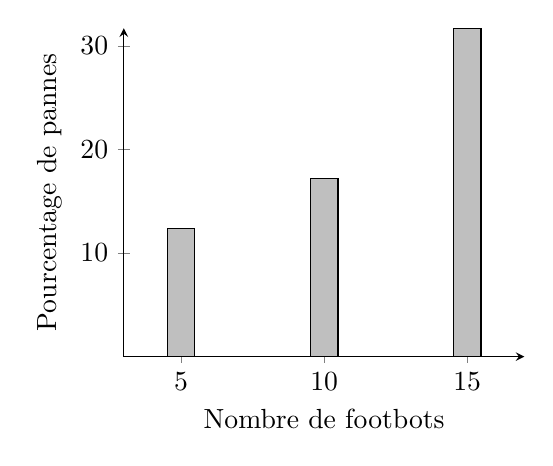
\begin{tikzpicture}
\begin{axis}[width=0.55\textwidth,
symbolic x coords={5,10,15},
xtick=data,
xlabel=Nombre de footbots,
ylabel=Pourcentage de pannes,
ymin=0,
ytick={10,20,30},
      axis x line=bottom,
      axis y line=left,
            enlarge x limits=0.2,
]
\addplot[ybar,fill=black!25] coordinates {
(5,   12.4)
(10,  17.2)
(15,   31.7)
};
\end{axis}
\end{tikzpicture}
\caption{Pourcentage de pannes de batterie après 10.000 steps, selon le nombre de robots}
\end{figure}

\FloatBarrier

\subsection{Performances Générales}



\section{Perspectives d'amélioration}

\subsection{Optimisation des constantes utilisées}
Tout au long de ce rapport, différents paramètres numériques ont été mis en avant et le comportement Lua a aussi été écrit de manière à ce que ces valeurs soient facilement accessibles. Il en résulte un ensemble de variables globales qui régissent toutes un aspect du comportement du robot dans l'expérience.

\begin{lstlisting}[caption=Définitions des variables globales]
--Specs received
BASE_SPEED=30
BATT_BY_STEP =.2

--Low-level
SCANNER_RPM=75
DIR_NUMBER = 15
EXPL_DIR_NUMBER = 20
EXPL_CONV = 3

--"Mid"-level:Movement
CONVERGENCE=1
OBSTACLE_PROXIMITY_DEPENDANCE=.25
OBSTACLE_DIRECTION_DEPENDANCE=.25
EMER_DIR_DEP=1
EMER_PROX_DEP=1
MIN_SPEED_COEFF = 0.6
--When a footbot "hits" something, he will pick a
--temporary speed between this coeff and 1 times BASE_SPEED
RANDOM_SPEED_TIME = 30
--The number of steps during which
--the footbot keeps this new random speed

--High-level:Decision Making
ORGN_SRC_DST=80
--Minimal distance between two sources considered "different"
MINE_PROB_WHEN_SRC_RECVD=.2
--Probability of starting mining upon receiving a new source
INIT_BATT_SEC=25
--Initial battery handling security coeff
IDEAL_NEST_BATT=20
--Leftover battery a footbot should have when returning to the nest
EPSILONGREED=0.1
--epsilon for epsilon-greedy choice algorithm
\end{lstlisting}

L'étape suivante consisterait à trouver une combinaison de ces variables qui maximise la performance des robots. Ceci est bien évidemment une problématique très vaste, d'une part parce que cette combinaison optimale de valeurs dépend de la manière dont la performance est mesurée et de la configuration d'expérience utilisée, et d'autre part parce que le nombre de ces variables est trop déraisonnablement élevé pour se lancer dans une telle optimisation sans d'abord essayer de simplifier le problème. Dans cette section, nous allons brièvement rappeler les paramètres qui sont apparus, montrer quelles sont les constantes qui jouent les rôles les plus importants et quelles possibilités immédiates d'adaptation notre comportement offre à travers la modification de ces variables globales.

Les constantes sont réparties en trois groupes: les constantes <<bas-niveau>>, les constantes utilisées par les différents algorithmes de déplacement, et les constantes <<haut-niveau>> qui interviennent dans la prise de décision. Parmi les constantes <<bas-niveau>>, on trouve la vitesse angulaire du \emph{distance scanner}, le nombre de directions dans lesquelles les mesures de ce capteur sont regroupées ainsi que la convergence $\kappa$ utilisée pour les <<rebonds>> lors de l'exploration\footnote{voir listing \ref{list:gaslike}.}. Ces constantes jouent un rôle extrèmement mineur et sont plutôt liées à la physique des footbots.

Dans les constantes liées au mouvement, on retrouve la convergence $\kappa$ utilisée dans le reste des situations ainsi que les deux paires de paramètres $\alpha$ et $\beta$ qui sont apparus dans l'évitement d'obstacles proches en \ref{sec:emerAvoid} et l'évitement intermédiaire en \ref{sec:mediAvoid}\footnote{Pour rappel, ces deux évitements sont les mêmes aux constantes et à la portée des capteurs utilisés près}. On retrouve aussi les paramètres utilisés pour introduire une composante aléatoire à l'évitement dans l'annexe \ref{appsec:randomAvoidance}. Ces constantes influent sur la qualité générale du mouvement à travers toute l'expérience, et il existe probablement une plage de valeurs qui optimisent le mouvement dans l'écrasante majorité des configurations. En d'autres termes, elles ne permettent pas d'adapter le comportement des footbots d'une situation a une autre.

Dans les constantes <<haut niveau>> liées à la prise de décision, on retrouve la distance minimale entre deux sources pour qu'elles soient considérées comme originales, la probabilité qu'un footbot commence à miner les ressources qu'il connaît lorsqu'il reçoit une nouvelle source, le coefficient de sécurité initial utilisé dans la gestion de l'autonomie, le résidu de batterie idéal que doit avoir le robot lorsqu'il rentre au nid pour se ravitailler, ainsi que la valeur du $\varepsilon$ utilisé dans la décision $\varepsilon$-greedy. Ces variables ont elles une influence majeure sur le comportement final des robots. Tout travail d'optimisation ultérieur devrait se pencher en priorité sur ces constantes-ci.

Parmi ces variables, il est cependant possible de mettre {\ttfamily INIT\_BATT\_SEC} à part car comme son nom l'indique il ne s'agit que du coefficient de sécurité initial puisqu'il est ensuite réévalué constamment durant l'expérience. Il suffit donc de lui donner une valeur largement supérieure à la normale et celle-ci sera abaissée au cours de l'éxécution. Pour jouer sur la prise de risque liée à la gestion de la batterie, il faut utiliser {\ttfamily IDEAL\_NEST\_BATT}.

{\ttfamily ORGN\_SRC\_DST} et {\ttfamily MINE\_PROB\_WHEN\_SRC\_RECVD} sont assez étroitement liées. L'influence de {\ttfamily ORGN\_SRC\_DST} est assez claire, mais lorque cette constante est modifiée, il faut penser à modifier {\ttfamily MINE\_PROB\_WHEN\_SRC\_RECVD} en parallèle. En effet, pour un même nombre de sources <<réellement différentes>> abaisser la première de ces constantes augmente le nombre de sources <<différentes selon les robots>> à découvrir et il est donc judicieux d'augmenter par la même occasion la tendance à l'exploration par le biais de {\ttfamily MINE\_PROB\_WHEN\_SRC\_RECVD}. De même, il peut être judicieux de jouer sur cette dernière constante si l'on dispose d'informations sur le nombre de sources réelles ou selon le but de l'expérience: rendement court-terme, rendement long-terme, découverte d'une proportion maximale des ressources,~\ldots\ Cependant, l'importance de ces deux variables peut-être réduite si l'on implémente les deux transitions supplémentaires proposées dans le diagramme \ref{fig:genFlowchart}.

Enfin, l'influence de $\varepsilon$ dans la décision $\varepsilon$-greedy est assez claire et bien documentée (voir par exemple \cite{foraging}.). Etant donné les résultats des études statistiques, une valeur plus élevée que celle utilisée ($0.1$) semble peut-être judicieuse, à moins qu'une refonte totale du choix de la source à exploiter ne soit nécessaire.

\subsection{Amélioration plus fondamentales (??)(This is bad)}

TODO

